
\input preamble.tex
\vskip 5pt

\vskip 5pt
\begin{center}
	\huge
	\textbf{Læringsoppdrag målesystemer for nivå - Stasjon 09}
	\normalsize
\vskip 5pt 
\end{center}

$$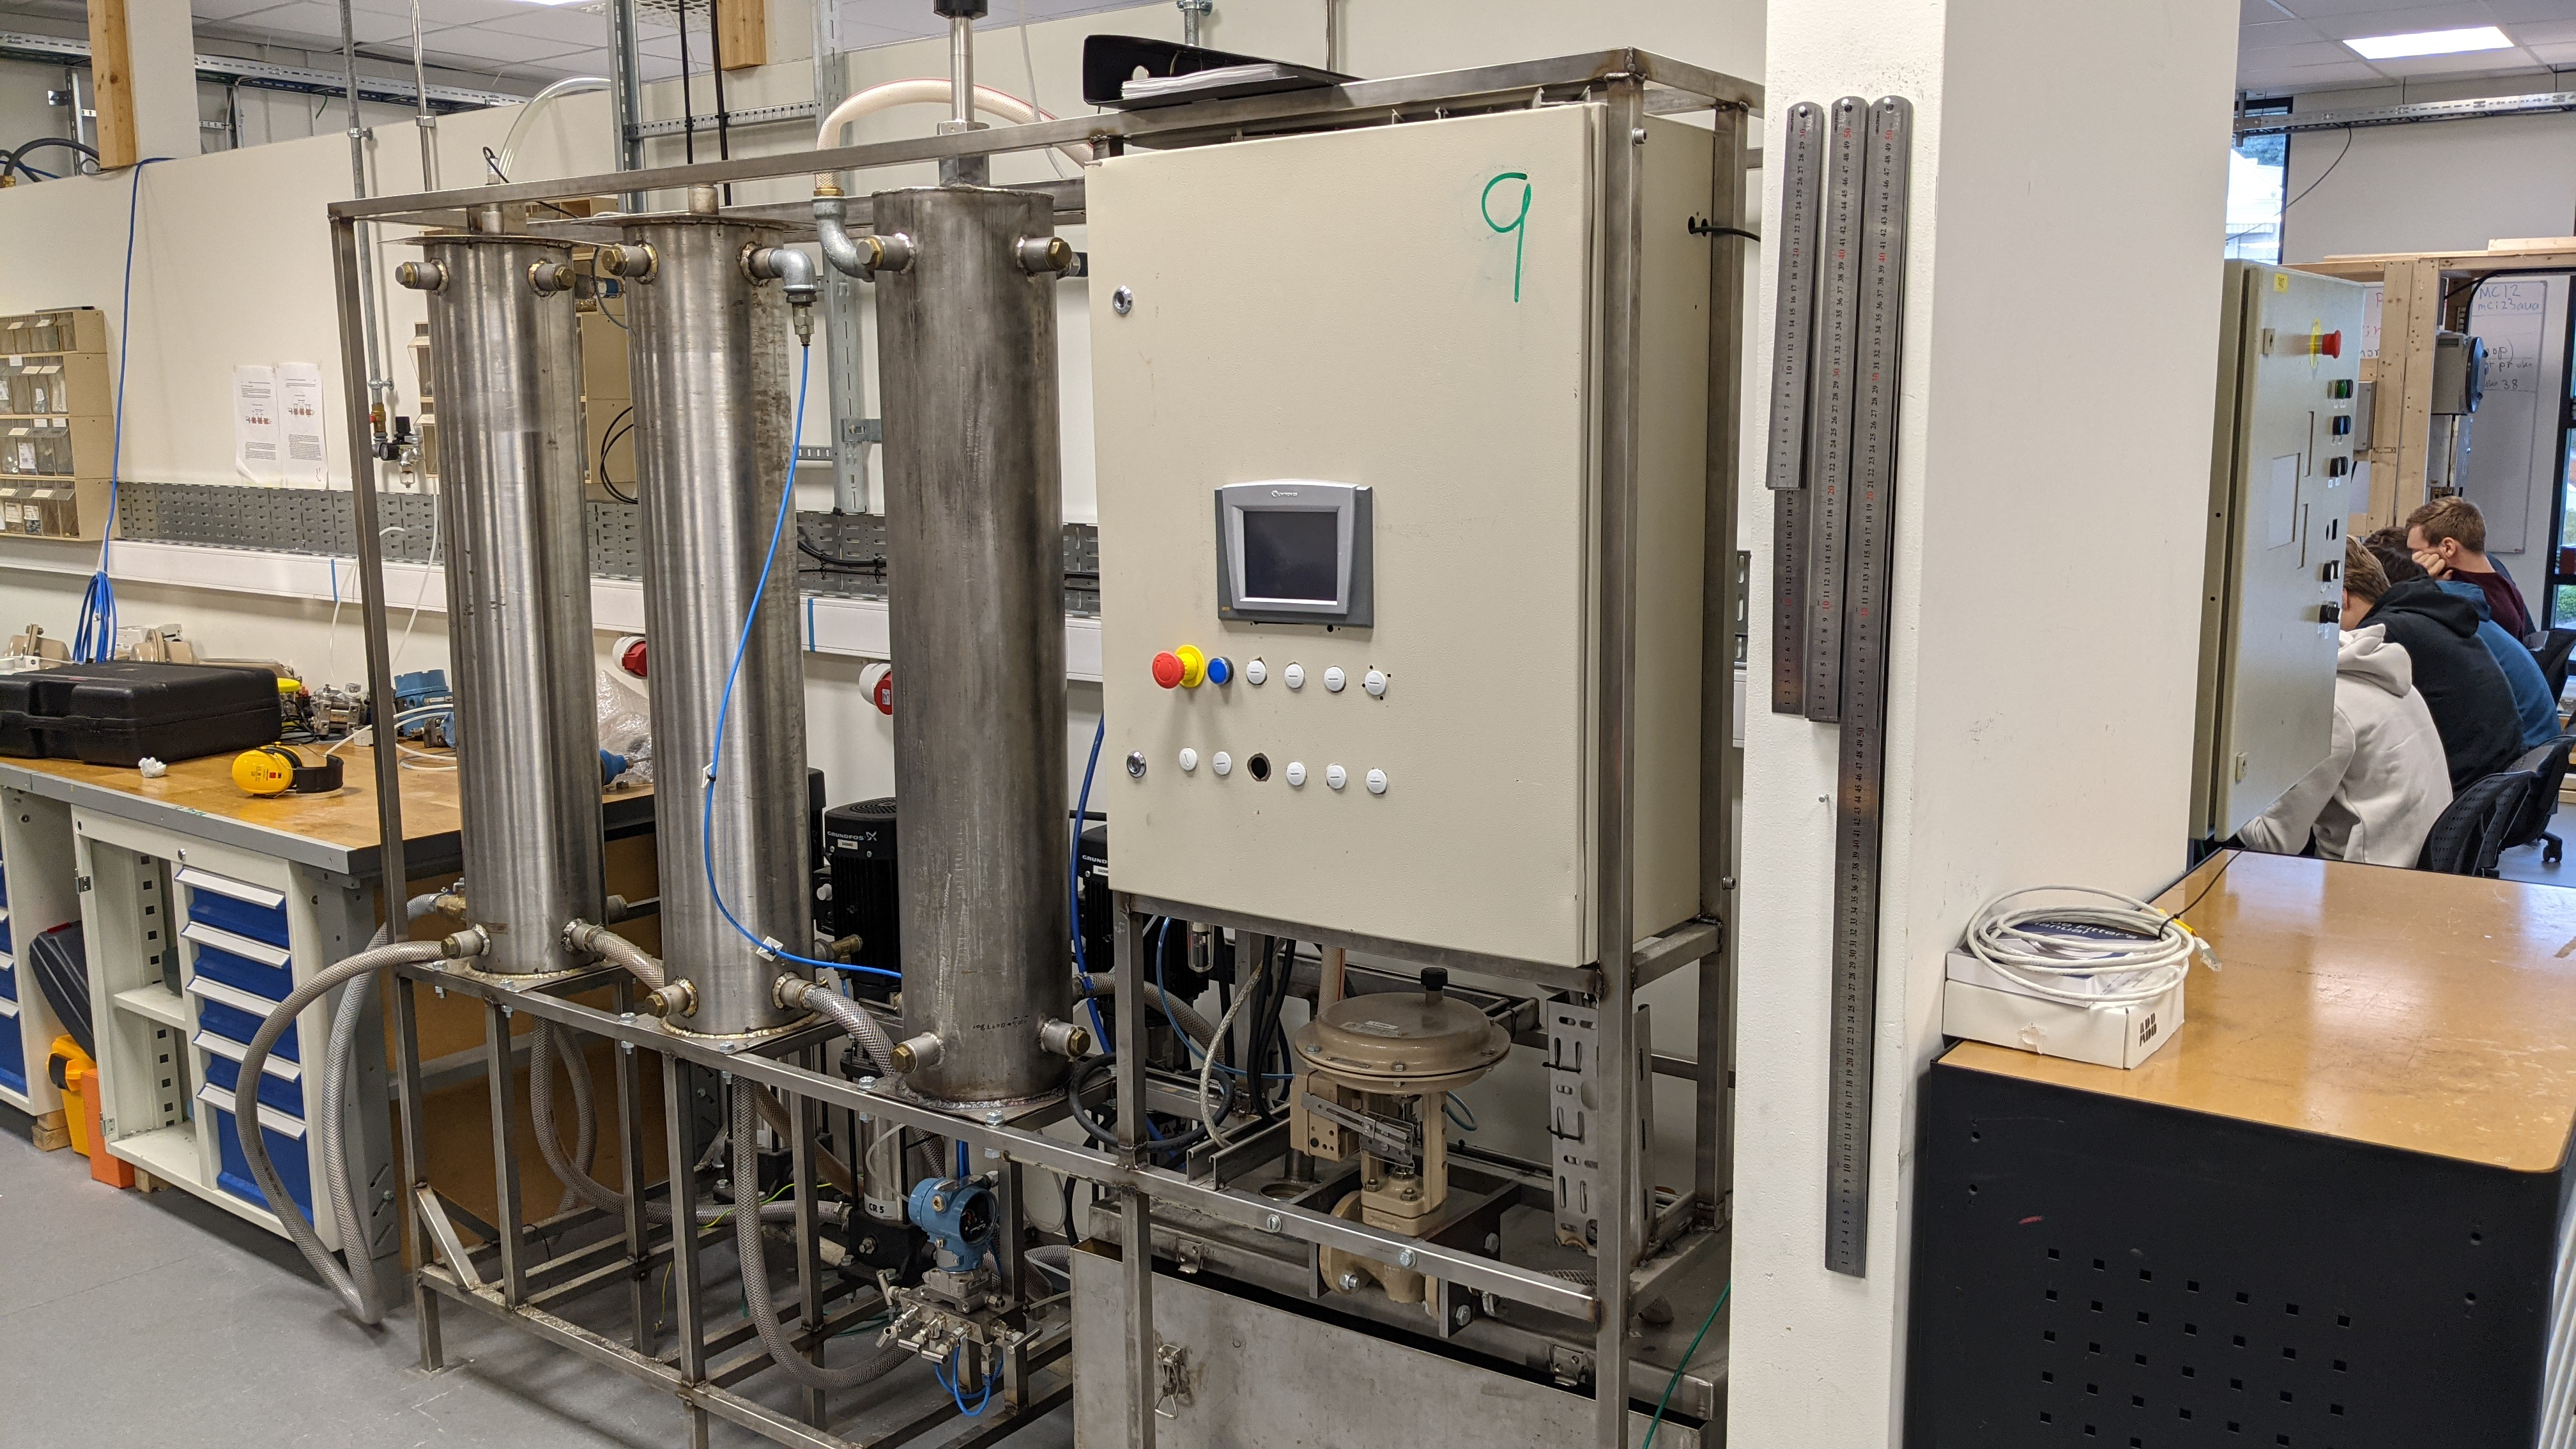
\includegraphics[width=13cm]{./stasjon09x01.jpg}$$\\

\vskip 1cm
Dette læringsoppdraget består av følgende:

\begin{itemize}[noitemsep]
	\item Oppgavesett nivå
	\item Arbeidsoppdrag målesystemer for nivå
\end{itemize}


 
\vskip 5pt 

Du kan jobbe parallelt med alle oppgavene. 

\vskip 5pt 
\textbf{Bakgrunnsteori}
 I filen \href {https://autofaget.no/pdfs/afgv.pdf}{afgv.pdf} er følgende kapittler til hjelp for dette læringsoppdraget:
 \begin{itemize}[noitemsep]
	 \item Kontinuerlig nivåmåling 
 \end{itemize}
\newpage
\textbf{Arbeidsoppdrag på stasjon 09}

\vskip 1cm

\textbf{Introduksjon}

I dette arbeidsoppdraget skal du jobbe med målesystemer for nivå. Du skal utføre sjekk og kalibrering for nivåmålesystemer basert på følgende prinsipper:
\begin{itemize}[noitemsep]
	\item Ultralyd
	\item Trykk
	\item Radar
\end{itemize}
Du skal sette i stand målesystemene for nivå på de tre tankene på denne stasjonen. Alt må koblet opp og virke mot stasjonens styresystem. 


\vskip 5pt 
\end{document}
